\chapter{Machine Learning}
\begin{center}
\begin{tcolorbox}[enhanced,width=6in,center upper,
    fontupper=\large,drop fuzzy shadow southwest,
    colframe=blue!50!black,colback=blue!10]
Für dieses Unterkapitel ist ein Jupyter-Notebook verfügbar. Siehe \gitresource{Machine Learning.ipynb}  
\end{tcolorbox}
\end{center}

\section{Grundzüge von Machine Learning}
Das Ziel von Machine Learning (ML) ist die Reproduktion von biologischem Lernverhalten in Computern. 
Ein Beispiel aus der Objekt-Klassifizierung: Menschen können schnell eine Lampe von einem Buch unterscheiden, obwohl es sehr viele verschiedene Lampen und Bücher gibt. 
Es ist allerdings schwierig, eine formelle Definition von \textit{Lampe} zu geben und somit Algorithmen zu entwerfen. 
Wir Menschen treffen solche Entscheidungen nicht mithilfe von solchen Definitionen, sondern wir benutzen unsere vorherigen Erfahrungen. Eine Lampe ist eine Lampe, weil es unsere vorherigen Erfahrungen mit Lampen widerspiegelt.\\

Da Computer keine Erfahrungen sammeln wie Menschen, brauchen wir eine Methode, um Computern etwas zu beizubringen. 
Wir müssen folgendes für den Computer bereitstellen:
\begin{enumerate}
    \item \textbf{Datensatz: } z.B. Bilder von Lampen
    \item \textbf{Modell: } in der Biologie ist dies das Gehirn
    \item \textbf{Verlustfunktion: } ein Mass dafür wie falsch die Aussagen sind.
\end{enumerate}
Wenn wir diese haben, können wir den Computer trainieren und dann validieren. 

\subsection{Datensatz}
Ein Datensatz ist eine Tabelle mit beliebig vielen Merkmale und einem Klassifizierungslabel (\textit{class label}=. Die Merkmale können Antworten zu ja-nein-Fragen oder aber auch Zahlen sein. Die Merkmale für eine Lampe können yum Beispiel die folgenden sein:
\begin{itemize}
    \item Ist es hell?
    \item Kann man es aus- und einschalten?
    \item Verwendet es Elektrizität?
\end{itemize}
Das class label ist dann: Ist es eine Lampe?
Wir werden ein Modell so trainieren, dass es aus den Merkmale das class label vorhersagen kann. 

\subsection{Modell}
Ein Modell ist eine Menge von möglichen Algorithmen, die die Merkmale als Argument nehmen und ein class label als Antwort zurückgeben. Wir beschriften diese Menge oft $\mathcal{H}$. Beispiele sind Entscheidungsbäume oder Neuronale Netze bestimmter Struktur  

\subsection{Verlustfunktion}
Eine Verlustfunktion $L(D,f)$ ist eine Funktion, die einen Datensatz D und eine $f \in \mathcal{H}$ als Argument nimmt und die Fehlerrate der $f$ in $D$ quantifiziert. Für Entscheidungsbäume wäre der Anteil von falschen Klassifizierungen eine mögliche Verlustfunktion. Es gibt keine allgemeine Verlustfunktion, sondern man muss eine für das Modell $\mathcal{H}$ eine auswählen.

\subsection{Training}
Das Training minimiert die Verlustfunktion anhand von Trainingsdaten. Wie man dies spezifisch schafft, ist abhängig von dem Modell und der Verlustfunktion. Es ist oft in Python Packages für verschiedene Modelle implementiert.

\subsection{Validierung}
Für Validierung verwenden wir einen anderen Datensatz $D'$ (also nicht den Trainingsdatensatz und überprüfen, dass die von Training ausgewählte $f^* \in \mathcal{H}$ auch für andere Datensätze funktioniert. Es kann sein, dass unser Modell nur die Datensatz D auswendig gelernt hat und keine Aussagen über andere Datensätze machen kann. Wie müssen deshalb sicherstellen, dass dies nicht der Fall ist.
\section{Ausgewählte Modelle}\label{ml:modelle}
\subsection{Entscheidungsbäume}
Entscheidungsbäume sind eine einfache Art, Datensätze mit binären Merkmalen zu klassifizieren. Sie bestehen aus einer Wurzel, Knoten und Blättern. 
Wurzeln und Knoten sind immer mit zwei Knoten oder Blättern verbunden und fragen immer nach einem bestimmten Merkmal in dem Datensatz. Abhängig von der Antwort wird man nach links oder nach rechts verwiesen. Die Konvention ist, dass eine ja-Antwort nach rechts und eine nein-Antwort nach links führt. Blätter sind die Enden vom Baum und geben  an, welches class label zu dieser spezifischen Kombination von Merkmalen gehört. Am besten stellt man sie grafisch dar ( z. B. Abb. \ref{fig:ml-baum}).\\

\begin{figure}[h]
    \centering
    \includegraphics[scale=0.4]{Figures/ML-Baum.png}
    \caption{Muster-Entscheidungsbaum aus der Vorlesung.}
    \label{fig:ml-baum}
\end{figure}

Da Bäume theoretisch unendlich lang sein könnten, setzt man vorher eine Tiefe fest. Die Tiefe ist einfach die maximal erlaubte Anzahl von hintereinander gelegten Knoten. Wie man eine gute Tiefe wählen kann, werden wir später sehen.\\

Eine praktische Verlustfunktion für Entscheidungsbäume ist:
\begin{equation}
    L(D,f) = \frac{\mathrm{Anzahl ~falsch ~klassifizierte ~Elemente ~in ~D}}{\mathrm{Anzahl ~Elemente ~in ~D}}~.
\end{equation}
\subsection{Lineare Regression}
Lineare Regression verwenden wir, wenn sowohl die Merkmale als auch die class labels  Zahlen sind. 
Für $n$ Merkmale ist unser Modell die Menge von allen $n$-dimensionalen Linearformen. 
Die Vorhergesagte class label $y$ ist dann die Linearform angewendet auf die Merkmale.

\begin{equation}
    \mathcal{H} = \left\{ y=f(x_1,...,x_n) = \sum_{i=1}^n w_ix_i ~~|~w_1,..,w_n \in \mathbb{R}\right\}
\end{equation}

Die Verlustfunktion (auch \textit{Mean Squared Error} gennant) ist dann:
\begin{equation}
    L(D, f) = \mathrm{MSE}(D,f) = \frac{1}{m} \sum_{i=1}^m (f(x_{1,i},...,x_{n,i}) - y_i)^2
\end{equation}
wobei $m$ die Anzahl von Zeilen in $D$ und $(x_{1,i},...,x_{n,i},y_i)$ die Zeilen des Datensatzes sind.\\

Um einzuschätzen, wie gut die Regression ist, bestimmen wir den \textbf{R2}-Wert eines Schätzers $f \in \mathcal{H}$. Wir definieren zuerst eine $f_0 = \frac{1}{n}\sum y_i$, der immer den Mittelwert der Trainingsdaten zurückgibt. Die R2-Score ist dann:
\begin{equation}
    R2(D,f) = 1 - \frac{\mathrm{MSE}(D,f)}{\mathrm{MSE}(D,f_0)}
\end{equation}


Ein negativer R2-Wert bedeutet, dass die Schätzer schlechter ist, als einfach immer den Mittelwert zurückzugeben. Je näher der R2-Wert an 1 ist, desto besser ist f. 

\subsection{Logistische Regression}
Logistische Regression wird verwendet, wenn man ein binäres class label und skalare Merkmale hat. Eine grafische Darstellung ist das Teilen des kartesischen Koordinatenraums in zwei Gebiete (siehe Abb. \ref{fig:ml-div}).

\begin{figure}[h]
    \centering
    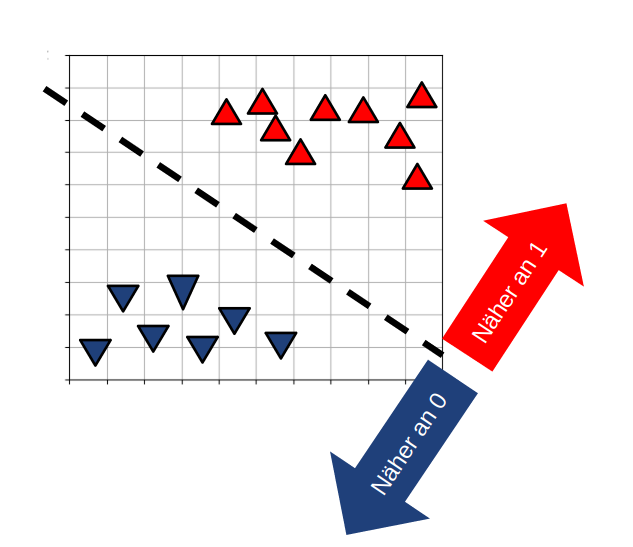
\includegraphics[scale=0.27]{Figures/ML-divided space.png}
    \caption{Beispiel für logistische Regression aus der Vorlesung.}
    \label{fig:ml-div}
\end{figure}

Dafür verwenden wir das Modell:
\begin{equation}
        \mathcal{H} = \left\{ y=f(x_1,...,x_n) = \sigma{w_0 + w_1*x_1 + ... + w_n*x_n} ~~|~w_0,..,w_n \in \mathbb{R}\right\}
\end{equation}
wobei  $\sigma$ die Sigmoidfunktion $\sigma: \mathbb{R} \to (0,1)$ ist. \footnote{Die Verlustfunktionen sind mathematische Normen für den Funktionenraum $L^2$ (nicht Klasurrelevant, für mehr Information MMP I)}

\section{Einschub: Under- und Overfitting}
In diesem Einschub werden wir Entscheidungsbäume näher betrachten. Wir möchten besonders den Einfluss von \textit{Tiefe} auf dem Erfolg des Modells verstehen.\\ 

Es gibt zwei mögliche Fälle:
\begin{enumerate}
    \item \textbf{Underfit: } Die Tiefe war zu klein, sodass das Modell nicht genügend lernen könnte.
    \item \textbf{Overfit: } Die Tiefe war zu gross. Das Modell hat den Datensatz auswendig gelernt. Wir haben nur den Datensatz auf dem Format von einem binären Baum umgeschrieben.
\end{enumerate}
Das ideale Modell hat eine Tiefe, die weder zu groß noch zu klein ist. Die einfachste Methode, diese Tiefe zu finden, ist, verschiedene Tiefen zu ausprobieren. 

Sei $D$ der Datensatz, $\mathcal{H}_n$ Entscheidungsbäume der Tiefe $n$, und $f_{n,D^*} \in \mathcal{H}_n$ der Baum, der eine Verlustfunktion auf $D^*$ minimiert. Mit den folgenden Methoden kann man eine gute Tiefe finden.
\subsection{Crossvalidation} \label{ML-Crossval}
\begin{enumerate}
    \item Teile D in ein \textit{training} Dataset $D^*$ und ein \textit{validation} Dataset $D'$. Oft ist das Training-Dataset länger. 
    \item Wähle Tiefen $t_1,...t_i$, die untersucht werden sollen.
    \item Finde $f_{t_1,D^*},...,f_{t_i,D^*}$ durch das Training und berechne $L(D',f_{t_1,D^*}),...,L(D',f_{t_i,D^*})$
    \item  Die Tiefe mit dem minimalen Verlustwert in 3. ist die optimale Tiefe.

\end{enumerate}
\subsection{k-Fold Crossvalidation}
\begin{enumerate}
    \item Teile $D$ in $k$ gleichlange Teile. Wir nennen diese $D_1,...,D_k$. 
    \item Für jedes $D_i$ führe crossvalidation \ref{ML-Crossval} mit $D_i$ als \textit{validation} Dataset und Rest von D als \textit{training} Dataset. 
    \item Die Tiefe, die am häufigsten den minimalen Verlustwert hatte, ist die optimale Tiefe. 
\end{enumerate}

\section{Neuronale Netze}
\textit{Neuronale Netze} bezeichnet ein Modell, das direkt von  biologischen Strukturen inspiriert ist. Ein Neuron im ML-Sinne  besteht aus gewichteten Eingängen und einem Ausgang. Die Neuronen sind in neuronalen Netzen in Schichten organisiert. Die Ausgänge von den Neuronen in einer Schicht sind die Eingänge der Neuronen in nächster Schicht.\\
\begin{figure}[h]
    \centering
    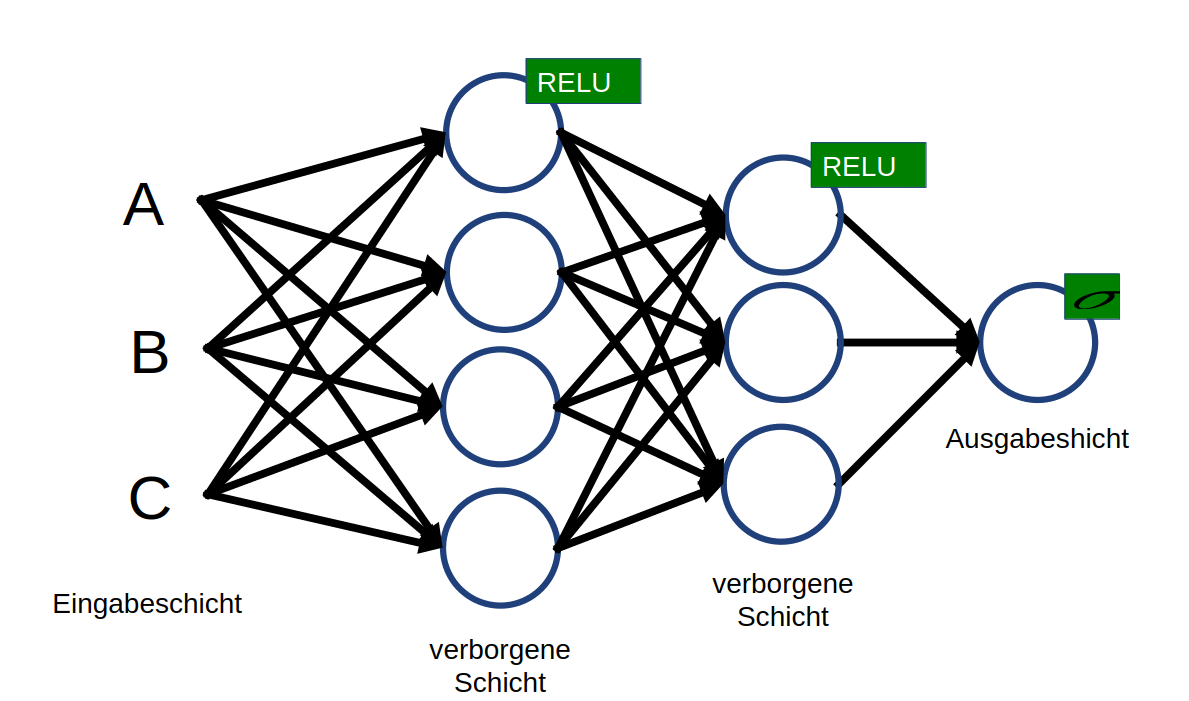
\includegraphics[scale=0.3]{Figures/ML-NNetz.png}
    \caption{Ein Beispiel für ein neuronales Netz. }
\end{figure}

Neuronen sind mathematisch folgenderweise konstruiert: 
\begin{equation}
    f(x_1,...,x_n) = a(c + w_1 x_1 + ... + w_n x_n)
\end{equation}
wobei $a$ eine Aktivierungsfunktion $a: \mathbb{R} \to \mathbb{R}$ ist. Häufig verwendete Aktivierungsfunktionen sind  in Tabelle \ref{ML:aktivierungsfunktionen} zu sehen. Die RELU wird heutzutage am meisten verwendet.\\

 
\begin{table}[h]
\centering
\begin{tabular}{lllll}
\cline{1-2}
\multicolumn{1}{|l|}{RELU}   & \multicolumn{1}{l|}{f(x) = max(0,x)}              &  &  &  \\ \cline{1-2}
\multicolumn{1}{|l|}{$\sigma$} & \multicolumn{1}{l|}{$f(x) = \frac{1}{1+e^{-x}}$}    &  &  &  \\ \cline{1-2}
\multicolumn{1}{|l|}{TANH}   & \multicolumn{1}{l|}{$f(x) = \frac{2}{1+e^{-2x}}-1$} &  &  &  \\ \cline{1-2}
                             &                                                   &  &  & 
\end{tabular}
\caption{Häufig verwendete Aktivierungsfunktionen.}
\label{ML:aktivierungsfunktionen}
\end{table}

Während Training sind die gewichte $c, w_1,...,w_n$ für jedes Neuron zu optimieren. Die Struktur von den Neuronen ist vorher zu finden.

\subsection{Convolutional Neural Networks}
Das Hauptziel von CNNs sind Bilderkennung. Wir möchten immer noch Objekte von einander unterscheiden, aber statt skalarer Merkmale möchten wir jetzt Bilder betrachten. Als erste Idee könnten wir jeden Pixel als Eingang zu einem neuronalen Netz nehmen und ein riesiges Netzwerk verwenden, um die Klassifikation durchzuführen. Aber dafür bräuchten wir zu viele Neuronen. Stattdessen verwenden wir \textit{convolution} \footnote{Convolution ist hier nicht im Sinne von \textit{Complex} (convoluted), sondern im Sinne von \textit{Faltung} zu verstehen. }, um die Bilder zu vereinfachen. Für Faltung betrachten wir Bilder als Matrizen. Sei $E \in \mathbb{R}^{nxn}$ die zu faltende Matrix und $F \in {0,1}^{2x2}$ die Faltungsmatrix. Der Ausgang ist $A \in \mathbb{R}^{n-1xn-1}$. \footnote{Falls $n$ keine ganzzahliges Mehrfaches von der Größe von $F$ ist, dann vernachlässigt man genügend der letzten Zeilen und Spalten von $E$.}
\begin{equation}
    A_{i,j} = E_{i,j}F_{1,1} + E_{i+1,j}F_{2,1} + E_{i,j+1}F_{1,2} +E_{i+1,j+1}F_{2,2}     
\end{equation}
Man stellt dies am besten grafisch dar: Man legt die Faltungsmatrix auf jeden 2x2 Block in $E$, multipliziert die Einträge, die aufeinander liegen, summiert die Ergebnisse, und notiert die Summe auf einer neuen Matrix für jeden 2x2 Block in $E$. \\

Man kann noch einen Filter (Aktivierungsfunktion) auf das Ergebnisse anwenden. Zum Beispiel:
\begin{equation}
        A_{i,j} = RELU( E_{i,j}F_{1,1} + E_{i+1,j}F_{2,1} + E_{i,j+1}F_{1,2} +E_{i+1,j+1}F_{2,2} )
\end{equation}

Eine weitere Methode, die für CNN verwendet wird ist \textit{Pooling}. Es wird ähnlich wie Faltung angewendet, aber es keine lineare Funktion, sondern \textit{max} oder \textit{min}:
\begin{equation}
    A_{i,j} = \mathrm{max}\{E_{i,j};E_{i+1,j};E_{i,j+1};E_{i+1,j+1}\}
\end{equation}

Eine geschickte Wahl von Faltungsschichten führt nicht nur zu einer Reduktion der Bilddimension, sondern auch zu Hervorhebung von Merkmalen (Kanten, Ecken etc.) des gesuchten Objekts (siehe Abb. \ref{fig:ml-conv}. Man kann die "gefalteten" Bilder dann mithilfe eines neuronalen Netzes klassifizieren.

\begin{figure}[h]
    \centering
    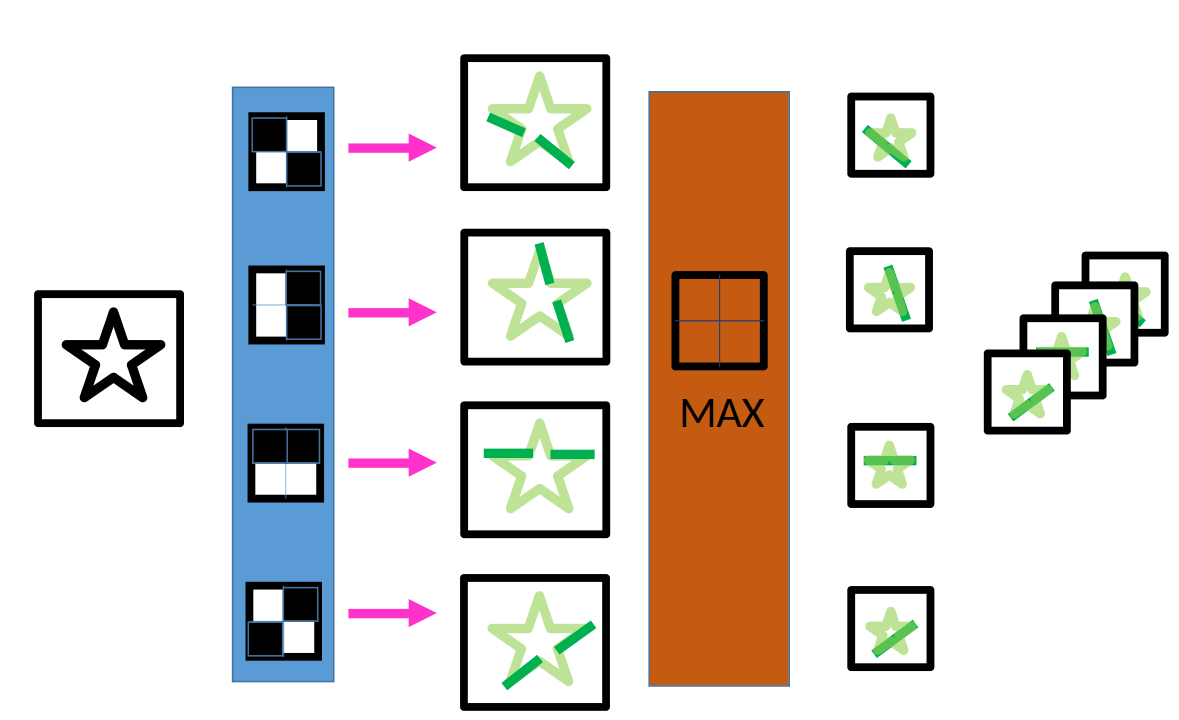
\includegraphics[scale= 0.3]{Figures/ML-conv.png}
    \caption{Hier werden die Kanten von einem Stern mit einem CNN hervorgehoben. Die nachfolgende neuronale Netze können dann aus dem Kanten entscheiden, ob es einen Stern ist.}
    \label{fig:ml-conv}
\end{figure}
\subsection{Andere Architekturen}
\subsubsection{Autoencoder}
Ein Autoencoder besteht aus einem Encoder und einem Decoder. Der Encoder überführt die Eingangsinformation (Bild oder Data) in einen mehrdimensionalen Raum (auch Code Space genannt). Der Decoder ist die umgekehrte Operation. Die Idee ist, dass ähnliche Eingänge näher zu einander im Code Space abgebildet werden. Dann können wir mithilfe von Clustering die Daten klassifizieren. Ein Beispiel ist Schrifterkennung. Bilder von Schriftzeichen werden mithilfe von einem Encoder auf dem Code Space abgebildet. Dann können wir aus der Position im Code Space erkennen, welches Schriftzeichen es war.\\

Der Encoder und Decoder sind neuronale Netze, die auch trainiert werden müssen. Die Layers sind Sanduhr artig, dies führt dazu, dass nur die wichtigste Information imm Code Space abgebildet wird. Was diese Information (bzw. was die Achsen von Code Space bedeuten) a priori unbekannt. Die Verlustfunktion für Training ist:
\begin{equation}
    L(D, enc,dec) = \sum_{x\in D} || x -Dec(Enc(x)||^2
\end{equation}

\subsection{Generative Adversarial Networks (GAN)}
GANs sind dafür geeignet, um Bilder zu generieren oder zu verändern. Ein GAN hat einen Generator, der Bilder generieren kann und einen Diskriminator, der Bilder beurteilen kann. Der Diskriminator versucht die Bilder vom Generator von echten Bildern unterscheiden zu können. Der Generator versucht Bilder, die vom Diskriminator als ``echt`` gesehen werden, zu generieren.

\section{Kodierung kategorischer Daten}
Wie wir gesehen haben, arbeiten alle bisherige Modelle auf numerischen Daten (entweder {0,1} oder $\mathbb{R}$), aber im reellen Leben sind Daten oft nicht numerisch, sondern kategorisch \footnote{z.B Gender wird oft mit männlich, weiblich oder divers bezeichnet. Diese lassen sich aber nicht natürlicherweise mit Zahlen ausdrücken. }. Deshalb müssen uns bewusst eine Codierung auswählen. In dem folgenden Paragrafen betrachten wir verschiedene Methoden anhand des Titanik-Dataset (siehe Abbildung \ref{fig:titanik-dataset}.

\begin{figure}
    \centering
    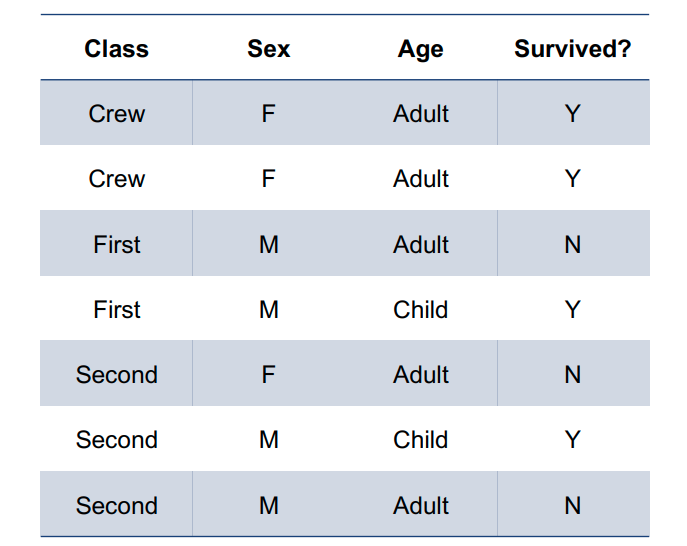
\includegraphics[scale=0.4]{Figures/Ml-Titanik-Dataset.png}
    \caption{Auszug des Titanik Datasets. }
    \label{fig:titanik-dataset}
\end{figure}
\subsection{Ordinal Encoding}
Dies ist die einfachste Methode. Mögliche Kategorien jedes Merkmals werden mit arbiträren ganzen Zahlen bezeichnet. Zum Beispiel im Titanik-Dataset können wir für das Merkmal \textit{class} Crew mit 1, First mit 2 und Second mit 3 bezeichnen. Obwohl wir die Zahlen willkürlich gewählt haben, haben wir plötzlich Crew näher mit First als mit Second platziert. Das kann  in der Auswertung nachteilig sein.

\subsection{Mean Encoding}
Hier bezeichnen wir jede Kategorie mit einem Mean, der mit Hilfe von dem \textit{class label} generiert wird. In unserem Fall können wir dieses Mean als Überlebenschance nehmen. Für \textit{Age} Merkmal bezeichnen wir \textit{Kind} mit 1, denn jedes Kind hat überlebt und \textit{Adult} mit 0.4, denn 40 \% der Erwachsene haben überlebt. Nachteil ist, dass wir plötzlich Information aus dem \textit{class label} in die Merkmale übertragen haben. Dies kann zu Overfitting führen.

\subsection{One-Hot Encoding}
Für diese Methode machen wir aus einem Merkmal mit $n$ Kategorien $n$ Merkmale, d.h. z. B. für das Merkmal \textit{class}: Es gibt jetzt drei Merkmale mit Werten {0,1}. Diese sind ''Ist Crew?'', ''Ist First?'' und ''Ist Second?''. Dadurch haben wir keinen der Nachteile der vorherigen Methoden, aber unser Datensatz ist \textit{viel}\footnote{Der Titanik-Datensatz hat nach One-Hot Encoding ca. 2 mal mehr Merkmale.} größer geworden. 


\section{Clustering \& K-Means-Methode}
Wir möchten unsere Daten mit skalaren Merkmalen (z.B. Helligkeit und Größe für Sterne) gemäß ihrer Entfernung zueinander in Clusters (Bündel) sammeln. Die k-Means-Methode dient dazu, die geeigneten Bündel zu finden. Unser Modell ist
\begin{equation}
     \mathcal{H} = \left\{ (\theta_1,...,\theta_k,c) | \theta_1,...,\theta_k \in \mathbb{R}^d \land c : \mathbb{R}^d \to \{1,...,k\} \right\}
\end{equation}
wobei wir k Bündel mit Mittelpunkt (auch Zentroid benannt) $\theta$ und die Zuweisungsfunktion $c$ betrachten. Die Funktion $c$ gibt für jeden Punkt in $\mathbb{R}^d$ an, zu welchem Bündel dieser Punkt gehört. Zu bemerken ist, dass dies kein neuronales Netz ist. Die Verlustfunktion ist so gedacht, dass der Abstand der Punkten zu ihrem zugewiesenen Cluster-Mittelpunkt bestraft wird. Wir formalisieren dies wie folgt:\\

$D \subseteq \mathbb{R}^d$ sind die gegebenen Punkte,  $\{\theta_1,...,\theta_k\} \subseteq \mathbb{R}^d$ die Cluster-Mittelpunkte, $c$ die Zuwesiungsfunktionen. Dann ist die Verlustfunktion: 
\begin{equation}
    \mathcal{L}(D,\theta_1,...,\theta_k,c) = \sum_{x \in D} || x - \theta_{c(x)}||^2 
\end{equation}
Bemerkung: $\theta_{c(x)}$ ist der  $x$ zugewiesene Mittelpunkt.\\

Für Training verwenden die folgende Algorithmus:

\begin{itemize}
    \item \textbf{Gegeben: } $D \in \mathbb{R}^d$
    \item \textbf{Initialisierung: } wähle $\theta_1,...,\theta_k$ zufällig. 
    \item \textbf{Zuweisung Aktualisieren: } wir setzen $c(x) = argmin_{j \leq k} || x -\theta_j||$. Dies bedeutet, dass jedem Punkt der nächstgelegene Cluster-Mittelpunkt zugewiesen wird.
    \item \textbf{Cluster-Mittelpunkte Aktualisieren: } Sei $S_j = \left\{ x \in \mathbb{R}^d | c(x) = j\right\}$ die Menge der Punkte in Cluster $j$. $\forall j \leq k$ setze $\theta_j = \frac{1}{|S_j|} \sum_{x \in S_j} x$. Somit haben wir alle Cluster-Mittelpunkte auf dem wirklichen Mittelpunkt des Clusters gesetzt.
    \item Führe die Aktualisierung-Schritte immer wieder durch, bis die Clusters sich nicht mehr ändern. 
\end{itemize}
\begin{figure}
    \centering
    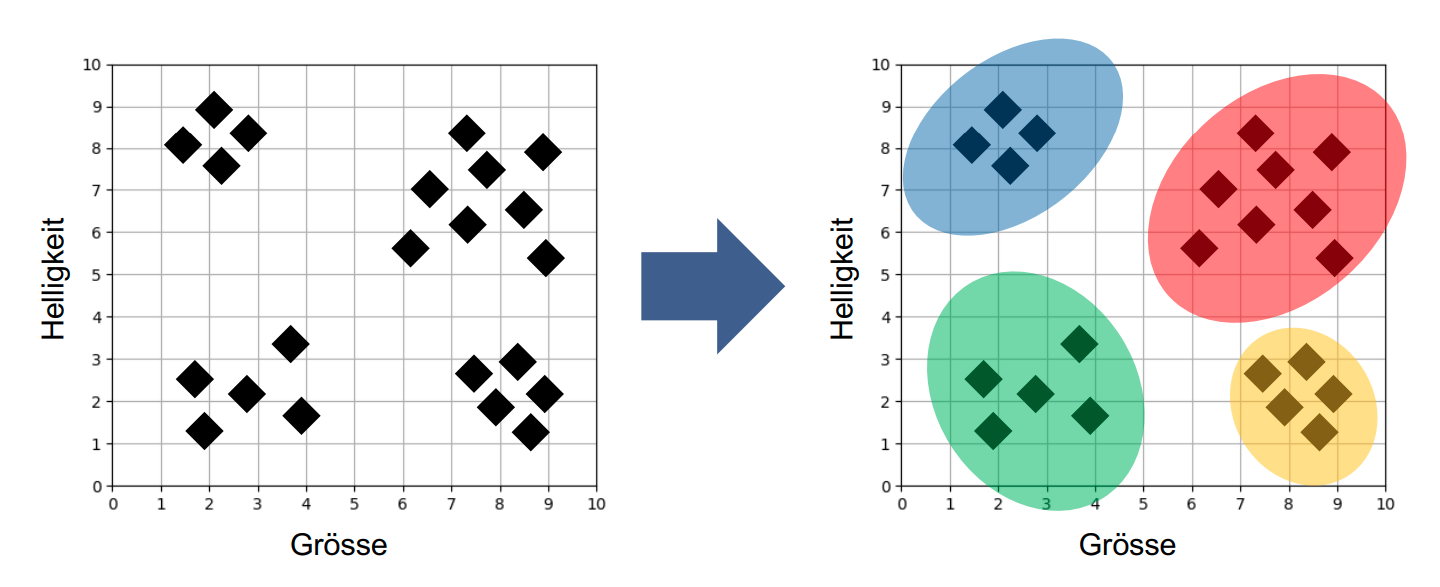
\includegraphics[scale=0.3]{Figures/ML-Clustering.png}
    \caption{Graphische Vorstellung des Clustering.}
\end{figure}
\subsection{Overfitting}
Wenn wir $k$ zu gross wählen (z.B  $k \geq |D|$), dann ist die beste Zuordnung immer einen Punkt pro Cluster. Wir können dies  nicht mit Cross-Validation (siehe \ref{ML-Crossval}) bemerken, denn $\mathcal{L}$ strebt gegen 0 für $k$ gegen $|D|$. Wenn wir mit Cross-Validation Overfitting verhindern wollen, dann müssen wir die Verlustfunktion so verändern, sodass sie auch große k bestraft. Wir verwenden mit $\lambda > 0$:
\begin{equation}
    L = \mathcal{L} + \lambda e^k
\end{equation}
Jetzt können wir Cross-Validation verwenden, um die optimale Anzahl Clusters zu finden. 

\section{Principal Component Analysis (PCA)}
Als Letztes betrachten wir die PCA, was dafür gedacht ist, die Dimension (Anzahl Merkmale) ohne große Verluste von Information zu reduzieren. Dies ist nützlich, weil so unsere anderen Modelle schneller und korrekter funktionieren, wobei besonders wichtig ist, dass sie korrekter werden. Mit einer hohen Anzahl von Merkmalen wird der Suchraum $\mathbb{H}$ größer und es kann sein, dass wir nicht die perfekte Lösung finden.

Formell ist PCA eine Methode unseren Datensatz $\{x_1,...,x_n\} \subseteq \mathbb{R}^D$\footnote{Die $x_i$'s sind die Zeilen des Datensatzes und  $D$ ist die Anzahl von Merkmalen. } auf einem reduzierten Datensatz $\{t_1,...,t_n\} \subseteq \mathbb{R}^d$ abzubilden. Aus Lineare Algebra Perspektive ist die PCA eine Abbildung auf einen Unterraum. Wir möchten allerdings  so viel Information wie möglich behalten. Die Abbildung wird $\forall i \leq n$ folgenderweise definiert:
\begin{equation}
    t_i = (x_i \cdot w_1 ,... x_i \cdot w_d)^T
\end{equation}
wobei $\{w_1,...,w_d\} \subseteq \mathbb{R}^D$ die Gewichtsvektoren sind. 

\textbf{\textit{Fall 1: d=1}}\\


In diesem Fall suchen wir nur die $w_1$, sodass $t_i = (x_i \cdot w_1) \in \mathbb{R}$ die  Streuung  $\sum t_i^2$ maximiert. Sei \textbf{X} die $n\times D$ Matrix, die in jeder Zeile ein Element aus dem Datensatz hat.

\begin{equation}
    X = \begin{pmatrix}
        - ~x_1~ -\\
        - ~ x_2 ~ - \\
        .\\.\\.\\
        -~x_n~-
        \end{pmatrix}\\
\end{equation}
Dann können wir $w_1$ mit Hilfe folgender Gleichung finden: 
\begin{equation}
    w_1 = argmax_{||w|| = 1}\left\{ \sum_i^n (x_i\cdot w_n)^2 \right\}= argmax_{||w|| = 1} \left\{||\textbf{X}w||^2\right\}
\end{equation}
Die Ausdruck $||\textbf{X}w||^2$ wird maximal, wenn $w$ der Eigenvektor $u_1^*$ zum größten Eigenwert $\lambda_1^*$ ist. Dies kann mit Methoden aus der linearen Algebra finden. \\

\textbf{\textit{Fall 2: $d \geq 1$}}\\

In diesem Fall suchen wir $d$ Gewichtsvektoren. $w_1$ ist wieder wie in Fall 1 zu finden, für die $w_2$ subtrahieren wir die Projektion von $x$ auf den Unterraum \textit{Spann}{$[w_1]$} von $x$ für jedes $x \in X $ also:
\begin{equation}
    X_1 = \{x - proj_{u_1}^* x | x \in x\} = \{x - (x \cdot u_1^*)u_1^* | x \in x\}
    \label{eq_ml_proj_set}
\end{equation}
Dann können wir noch einmal die Methode von Fall 1 (aber jetzt mit $X_2$ als Datensatz) anwenden, um $w_2$ zu bestimmen. Folglich können wir mit mehrmaligen Anwenden $(w_1,...,w_d)$ bestimmen. Formell geschrieben:

\begin{align}
    \textbf{X}_k &= \textbf{X} - \sum_{s=1}^{k-1} \textbf{X}w_s w_s^T\\ \label{eq_ml_mat_proj}
    w_k &=  argmax_{||w|| = 1} \left\{||\textbf{X}_k w||^2\right\}
\end{align}
Die Gleichung \ref{eq_ml_mat_proj} ist äquivalent zu mehrmaligen Anwenden von Gleichung \ref{eq_ml_proj_set}.
